\chapter{Melodische transformatie}
\label{hoofdstuk:MT}

\section{Inleiding}
In dit hoofdstuk zullen verschillende melodische transformaties besproken worden met hun voor- en nadelen. Deze transformaties zullen werken op melodielijnen die monofoon zijn. Deze melodielijnen zullen behandeld worden als een opeenvolging van noten (toonhoogtes) en het ritme zal na transformatie gewoon behouden blijven. Enkel de toonhoogte van een noot zal aangepast worden. Het ritme zal bij de transformaties die hier besproken staan ook geen invloed hebben op de transformatie van een noot. 

\subsection{Fibonacci}
De transformaties die hier als voorbeeld gegeven worden zullen vaak in een zekere vorm de rij van Fibonacci\cite{url:Fibonacci} bevatten. Dit komt omdat in een vroeg stadium van het onderzoek de vraag bestond of transformaties die voortgaan op de rij van Fibonacci een beter resultaat zouden bieden dan willekeurige transformaties. Dit omdat de rij van Fibonacci in de natuur zo nadrukkelijk aanwezig is dat ook redelijkerwijs de vraag gesteld zou kunnen worden of deze in de muziekwereld zo een invloed zou kunnen hebben. Dit bleek moeilijk hard te maken. Aangezien de resultaten ook zeker niet slechter waren en omdat het ook onderdeel van het onderzoek was, zijn deze transformaties gebaseerd op de rij van Fibonacci vaak gebruikt ter illustratie.

\subsection{Beschrijving van een transformatie}
De melodische transformaties die besproken worden in dit hoofdstuk gaan telkens beschreven worden aan de hand van een tabel. Deze tabel zal telkens een mapping van 8 waarden bevatten. de tweede rij zal altijd waarden tussen -5 en +6 bevatten die als betekenis hebben met welke waarde (namelijk de hoeveelheid halve tonen) een bepaalde noot verhoogd of verlaagd moet worden. 

Welke noot met welke hoeveelheid getransformeerd moet worden wordt dan telkens weergegeven via een waarde op de bovenste rij. Deze rij is ook telkens cyclisch modulo 8. Wanneer bijvoorbeeld zoals in tabel \ref{tabel:transformatie1} de index van de noot weergegeven wordt op de bovenste rij, dan zal de noot op positie 4 met 5 halve tonen verhoogd worden door de transformatie. Maar ook de noot op positie 12 zal met 5 halve tonen verhoogd worden omdat 12 ook 4 geeft als rest na deling door 8.

\subsubsection{Afronding naar de toonaard}
\label{sub:afronding}
In hoofdstuk \ref{OBM:RPK} werd reeds het RPK-model besproken. Dit model wordt gebruikt ter evaluatie van de transformaties. Bij de bespreking van dit model was een van de drie belangrijke kenmerken van een noot om de probabiliteit te bepalen de \textit{key}. Noten die in de toonaard voorkomen zijn zo veel waarschijnlijker om voor te komen dan noten die niet in de toonaard voorkomen. Deze noten, die niet in de toonaard voorkomen, klinken over het algemeen ook vals voor de luisteraar. 

Daarom is ervoor gekozen om na uitvoer van de transformaties nog een afronding door te voeren. Deze afronding bestaat erin om na de transformatie van een noot in de melodielijn, indien deze niet tot de toonaard behoort (en enkel dan), te verhogen of verlagen met een halve toon. De afronding zal zijn naar die noot van de twee die de hoogste probabiliteit heeft volgens het RPK-model. Deze twee noten zullen ook telkens beide wel tot de toonaard behoren. 

De transformaties zelf zullen theoretisch geen rekening houden met deze afronding. Met andere woorden, dit zal niet expliciet vermeld worden in de beschrijvingen van de transformaties. Het is echter wel belangrijk te weten dat dit wel degelijk altijd gebeurt. Vandaar dat het soms ook kan zijn dat het in een illustratie lijkt alsof een transformatie een halve toon te hoog of te laag uitgevoerd is voor een bepaalde noot. Dit is geen fout maar valt te verklaren door de zonet besproken afronding.

\section{Afbeelding afhankelijk van de positie}
\label{MT:positie}
\subsection{Beschrijving transformatie}
Een eerste, voor de hand liggende melodische transformatie is er eentje die een noot in een muziekstuk gaat transformeren enkel naargelang zijn positie in de melodielijn. De transformatie die ter illustratie dient van dit concept wordt beschreven in tabel \ref{tabel:transformatie1}. Zo zal de noot op positie 6 door deze transformatie met 1 halve toon verhoogd worden. De noot op positie 13 zal met 4 halve tonen verlaagd worden. 

\begin{table}
  \centering
  \begin{tabular}{c | c c c c c c c c }
    Index (mod 8) & 0 & 1 & 2 & 3 & 4 & 5 & 6 & 7 \\
    \hline
    \hline
    Verhoging & 1 & 1 & 2 & 3 & 5 & -4 & 1 & -3 \\
  \end{tabular}
  \caption{Transformatie afhankelijk van de positie van de noot.}
  \label{tabel:transformatie1}
\end{table}

\subsubsection{Voorbeeld}
In figuur \ref{figuur:voorbeeld_transformatie_1} wordt ter illustratie deze transformatie toegepast op een korte melodielijn. De bovenste lijn geeft de originele melodie weer, de onderste lijn geeft het resultaat weer na transformatie. Bij de twee melodielijnen staat bij elke noot telkens ook zijn representatie in halve tonen (modulo 12). Dit zodat het voor de lezer makkelijker te volgen is hoe de transformatie precies verloopt. 

Tussen de twee notenbalken wordt aangegeven welke sprong de transformatie oplegt aan de melodielijn. Zo zal het verschil in getalwaarde tussen overeenkomstige noten op de bovenste en de onderste notenbalk telkens gelijk zijn aan de waarde die hier aangegeven staat. Merk op dat dit voor de tweede en zevende noot in dit voorbeeld niet het geval is. Hier lijkt het verschil tussen de noten in de bovenste en onderste lijn telkens een halve toon kleiner dan deze zou moeten zijn. Dit komt door de afronding besproken in onderdeel \ref{sub:afronding} aangezien de noot met getalwaarde 8 (G$\sharp$/A$\flat$) niet tot de toonaard van het muziekstuk (Do groot) behoort.

\begin{figure}[!ht]
  \centering
  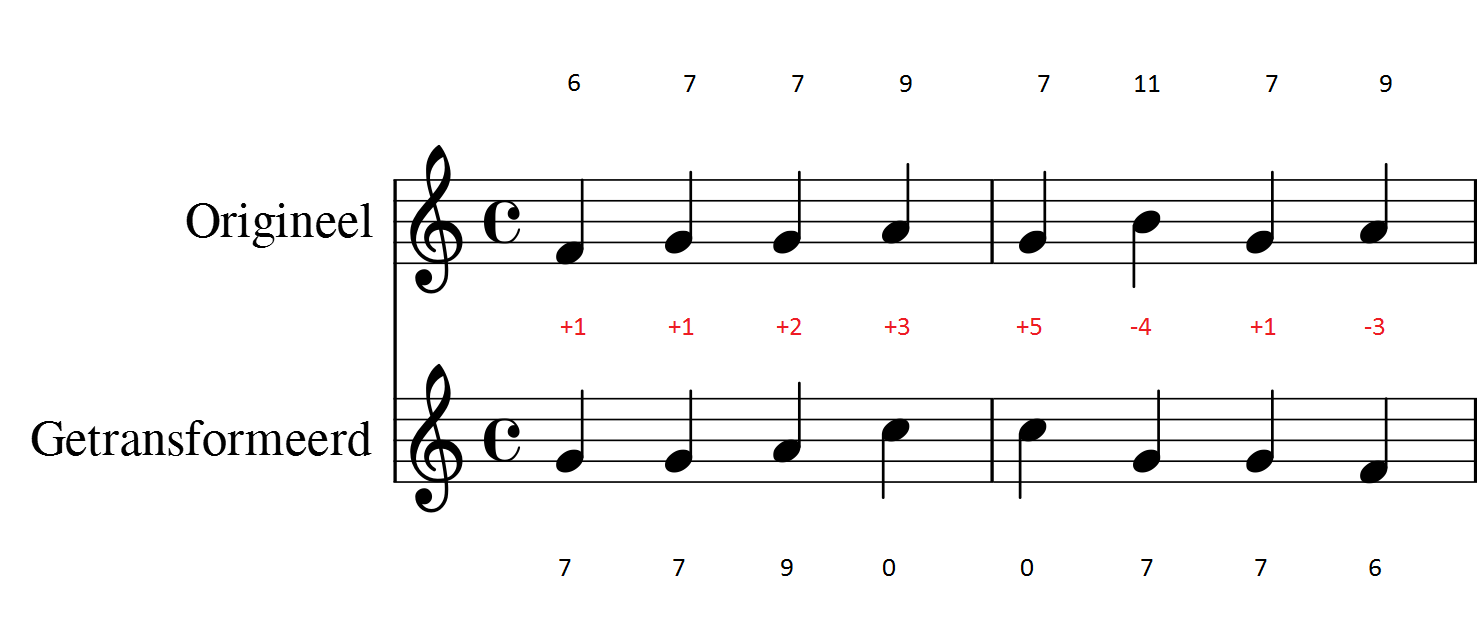
\includegraphics[width=0.75\textwidth]{3_Melodische_Transformatie/transfo1}
  \caption{Voorbeeld van toepassing transformatie afhankelijk van positie.}
  \label{figuur:voorbeeld_transformatie_1}
\end{figure}

\subsubsection{Bespreking transformatie}
Het grootste voordeel van deze transformatie is dat hij zeer eenvoudig uit te voeren en te begrijpen is. Enkel de positie van de noot is van belang met betrekking tot naar welke noot deze getransformeerd zal worden. Een groot nadeel van deze transformatie is dus ook dat deze totaal geen rekening houdt met de eigenlijke toonhoogte van de noot die getransformeerd gaat worden. Er wordt ook geen rekening gehouden met de context van de noot. Als er in het originele stuk patronen zitten zullen die ook nooit herkend en gelijk getransformeerd worden tenzij in het zeer specifieke geval dat deze telkens mooi op een veelvoud van 8 noten van elkaar voorkomen. 

Deze transformatie zal dus ook verder niet veel gebruikt worden. Het is interessant om deze transformatie te zien als een soort van \textit{baseline} voor een willekeurige transformatie, om dan andere transformaties mee te kunnen vergelijken. Ook kan het interessant zijn na te gaan of er veel verschil zit tussen zo een transformaties waarin grote sprongen zitten ten opzichte van transformaties waarin vooral kleinere sprongen zitten (aangezien deze het originele stuk minder zullen gaan vervormen).

\section{Afbeelding afhankelijk van de afstand ten opzichte van vorige noot}
\label{MT:afstand_vorige}
\subsubsection{Beschrijving transformatie}
Een andere melodische transformatie is er een die een noot in een muziekstuk gaat transformeren naargelang zijn afstand ten opzichte van de vorige noot in het muziekstuk. Hierbij zal er gekeken worden naar de afstand van de noot op positie $x$ in de originele melodielijn ten opzichte van de noot op positie $x-1$ in de nieuwe melodielijn (dit is dus de getransformeerde waarde van de vorige noot in het originele muziekstuk). De eerste noot van eender welk muziekstuk wordt in deze transformatie behouden omdat deze noot geen voorgaande noot heeft. 

Wat ook speciaal is aan deze transformatie is dat de verhoging die weergegeven wordt in de transformatietabel toegepast wordt in de tegengestelde richting van waar de huidige noot in de originele melodie staat ten opzichte van de vorige noot na transformatie. De transformatie die ter illustratie dient van dit concept wordt beschreven in tabel \ref{tabel:transformatie2}. 

Zo zal een noot die 2 halve tonen hoger ligt dan de getransformeerde waarde van de vorige noot met 1 halve toon verlaagd worden. Een noot die 6 halve tonen lager ligt dan de getransformeerde waarde van de vorige noot zal met 2 tonen verhoogd worden. Tot slot zal een noot die 1 halve toon lager ligt dan de getransformeerde toonhoogte van de vorige noot nog eens met 4 halve tonen verder verlaagd worden (omdat de waarde in de tabel negatief is).

\begin{table}
  \centering
  \begin{tabular}{c | c c c c c c c c }
    Diff (mod 8) & 0 & 1 & 2 & 3 & 4 & 5 & 6 & 7 \\
    \hline
    \hline
    Verhoging & 5 & -4 & 1 & -3 & 1 & 1 & 2 & 3 \\
  \end{tabular}
  \caption{Transformatie afhankelijk van de afstand van de huidige noot tot de vorige noot na transformatie.}
  \label{tabel:transformatie2}
\end{table}

\subsubsection{Voorbeeld}
In figuur \ref{figuur:voorbeeld_transformatie_2} wordt een voorbeeld gegeven van een korte melodielijn waarop deze transformatie wordt toegepast. Voor de eerste noot wordt er geen transformatie weergegeven, dat is omdat deze ook geen vorige noot heeft en dus niet getransformeerd wordt. 

Als we dan bijvoorbeeld naar de tweede noot kijken dan heeft deze getalwaarde 5, de vorige noot uit de getransformeerde melodie heeft waarde 7 dus het verschil is -2. De absolute waarde is 2 waardoor de sprong als grootte -4 heeft Aangezien het verschil negatief is moet deze waarde bij die van de noot opgeteld worden want we willen een sprong in de richting van de vorige noot. In dit geval zal de sprong toch de andere richting uit gaan aangezien de noot in de tabel zelf negatief is. Zo komen we normaal gezien uit op een noot met getalwaarde 1. Deze noot ligt niet in de toonaard en omdat de noot met getalwaarde 0 (die de grondtoon is van de toonaard) waarschijnlijker is dan die met waarde 2 wordt de noot met waarde 0 als getransformeerde noot gekozen. 

Als we dan verder gaan naar de volgende noot merken we dat het verschil met de getransformeerde van de voorgaande noot 4 halve tonen is. Een absolute waarde van 4 voor het verschil geeft aanleiding tot een sprong van grootte 1. aangezien het verschil positief is en de sprong in tegengestelde richting uitgevoerd moet worden, zal de sprong als waarde -1 hebben. En zo komen we na afronding bij een noot met getalwaarde 4 uit.

\begin{figure}[!ht]
  \centering
  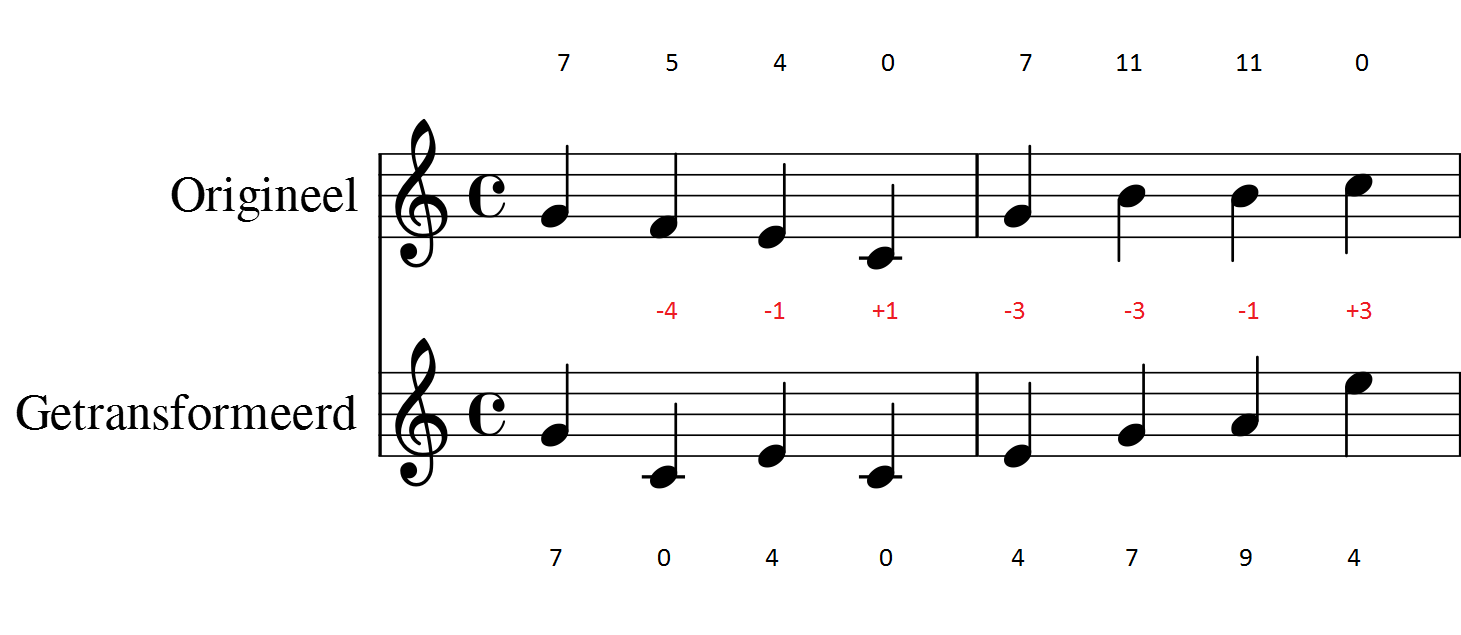
\includegraphics[width=0.75\textwidth]{3_Melodische_Transformatie/transfo2}
  \caption{Voorbeeld van toepassing van de transformatie afhankelijk van het interval ten opzichte van de vorige noot.}
  \label{figuur:voorbeeld_transformatie_2}
\end{figure}

\subsubsection{Bespreking transformatie}
Het interessante aan de transformatie die hier beschreven werd is dat deze de noten niet als losstaand beschouwt, maar ook de context gedeeltelijk in rekening brengt. Dit betekent dat eenzelfde noot naar zeer veel verschillende noten kan getransformeerd worden afhankelijk van de voorgaande noot. 

Een voordeel van deze transformatie is ook dat als er een zekere repetitiviteit in het originele muziekstuk zit, deze bijna altijd ook in het getransformeerde stuk zal voorkomen (enkel de noot die net voor zo een patroon voorkomt kan nog een extra invloed hebben). Dit maakt dat de structuur van het originele stuk nog iets meer bewaard blijft. 

Een nadeel van deze transformatie is dat deze wel nog steeds blind is voor de rest van de context. Ook de toonhoogte van de noot zelf heeft geen invloed op de grootte en richting van de transformatie op deze noot.  

%%% Local Variables: 
%%% mode: latex
%%% TeX-master: "masterproef"
%%% End: 
